\documentclass[10pt]{article}
\usepackage{hyperref}
\usepackage[utf8]{inputenc}
\usepackage{mathtools}
\usepackage{multicol}
\usepackage{amsmath}
\usepackage{graphicx}
\usepackage{array}
\usepackage[margin=0.5in]{geometry}
\usepackage{listings}
\usepackage{color}

\definecolor{mygreen}{rgb}{0,0.6,0}
\definecolor{mygray}{rgb}{0.5,0.5,0.5}
\definecolor{mymauve}{rgb}{0.58,0,0.82}

\lstset{ %
  backgroundcolor=\color{white},   % choose the background color; you must add \usepackage{color} or \usepackage{xcolor}; should come as last argument
  basicstyle=\footnotesize,        % the size of the fonts that are used for the code
  breakatwhitespace=false,         % sets if automatic breaks should only happen at whitespace
  breaklines=true,                 % sets automatic line breaking
  captionpos=b,                    % sets the caption-position to bottom
  commentstyle=\color{mygreen},    % comment style
  deletekeywords={...},            % if you want to delete keywords from the given language
  escapeinside={\%*}{*)},          % if you want to add LaTeX within your code
  extendedchars=true,              % lets you use non-ASCII characters; for 8-bits encodings only, does not work with UTF-8
  frame=single,	                   % adds a frame around the code
  keepspaces=true,                 % keeps spaces in text, useful for keeping indentation of code (possibly needs columns=flexible)
  keywordstyle=\color{blue},       % keyword style
  language=Octave,                 % the language of the code
  morekeywords={*,...},            % if you want to add more keywords to the set
  numbers=left,                    % where to put the line-numbers; possible values are (none, left, right)
  numbersep=5pt,                   % how far the line-numbers are from the code
  numberstyle=\tiny\color{mygray}, % the style that is used for the line-numbers
  rulecolor=\color{black},         % if not set, the frame-color may be changed on line-breaks within not-black text (e.g. comments (green here))
  showspaces=false,                % show spaces everywhere adding particular underscores; it overrides 'showstringspaces'
  showstringspaces=false,          % underline spaces within strings only
  showtabs=false,                  % show tabs within strings adding particular underscores
  stepnumber=2,                    % the step between two line-numbers. If it's 1, each line will be numbered
  stringstyle=\color{mymauve},     % string literal style
  tabsize=2,	                   % sets default tabsize to 2 spaces
  title=\lstname                   % show the filename of files included with \lstinputlisting; also try caption instead of title
}
\renewcommand{\arraystretch}{1.5}
\setcounter{secnumdepth}{0}
\author{Kevin Mambu}
\date{\today}
\title{M1 SESI 2017-2018\\Architecture Multi-Processeurs\\TP7 : Contrôleur DMA}
\setlength{\columnseprule}{1pt}
\def\columnseprulecolor{\color{black}}
\begin{document}
\begin{center}
  \texttt{\textbf{FPGA1 - Refcard}}
\end{center}
\begin{multicols}{2}
  \section{VHDL}
  \begin{itemize}
    \item RTL : Register Transfer Level
  \end{itemize}
  \begin{minipage}[t]{8cm}
    \begin{lstlisting}[language=VHDL]
    library ieee;
    use ieee.std_logic_1164.all;
    use ieee.std_logic_unsigned.all;
    entity MON-ET is
      generic (tp: time := 2ns);
      port( A : in std_logic;
      B : in std_logic;
      S : out std_logic);
    end entity MON-ET;
    architecture FLOT of MON-ET is
      begin
      s <= a and b after tp;
    end architecture FLOT;
    \end{lstlisting}
  \end{minipage}
  \subsection{Architecture structurelle}
  \begin{itemize}
    \item \texttt{and2 : entity work.MON-ET port map(A $\Rightarrow$ A,
    B $\Rightarrow$ B);}
  \end{itemize}

  \subsection{Comportemental}
  \begin{itemize}
    \item Process : réalisation de parties séquentielles
    \begin{itemize}
      \item Variables : abstraction algorithmiques
      \item !!! Signaux $\neq$ Variables !!!
    \end{itemize}
  \end{itemize}

  Conditionnelle IF :\\
  \begin{minipage}[t]{8cm}
    \begin{lstlisting}[language=VHDL]
      library ieee;
      use ieee.std_logic_1164.all;
      entity decodeur is
        port ( choix : in std_logic_vector(1 downto 0);
        decode : out std_logic_vector(3 downto 0));
      end entity decodeur;
      architecture comport of  decodeur
      decodage : process(choix) is
      begin
        IF (choix= "00") THEN decode <="0001";
        ELSIF (choix="01") THEN decode <="0010";
        ELSIF (choix="10") THEN decode <="0100";
        ELSE  decode <="1000";
        END IF;
      end process decodage;
      end architecture comport;
    \end{lstlisting}
  \end{minipage}\\
  Conditionnelle CASE :\\
  \begin{minipage}[t]{8cm}
    \begin{lstlisting}[language=VHDL]
    library ieee;
    use ieee.std_logic_1164.all;
    entity decodeur is
      port ( choix : in std_logic_vector(1 downto 0);
      decode : out std_logic_vector(3 downto 0));
    end entity decodeur;
    architecture comport of  decodeur
    decodage : process(choix) is
    begin
      IF (choix= "00") THEN decode <="0001";
      ELSIF (choix="01") THEN decode <="0010";
      ELSIF (choix="10") THEN decode <="0100";
      ELSE  decode <="1000";
      END IF;
    end process decodage;
    end architecture comport;
    \end{lstlisting}
  \end{minipage}\\
  Conditionnelle FOR :\\
  \begin{minipage}[t]{8cm}
    \begin{lstlisting}[language=VHDL]
    process (A)
    begin
    	Z <= "0000";
    	for I in o to 3 loop
    		if (A = I) then
    			Z(I) <= '1';
    		end if;
    	end loop;
    end process;
    \end{lstlisting}
  \end{minipage}\\
  Conditionnelle WITH/SELECT :\\
  \begin{minipage}[t]{8cm}
    \begin{lstlisting}[language=VHDL]
    with a select b <=
      "1000" when "00",
      "0100" when "01",
      "0010" when "10",
      "0001" when "11";
    \end{lstlisting}
  \end{minipage}\\
  Géneration generate :\\
  \begin{minipage}[t]{8cm}
    \begin{lstlisting}[language=VHDL]
    architecture GEN of REG_BANK is
      component REG
        port(D,CLK,RESET : in  std_ulogic;
             Q           : out std_ulogic);
      end component;
    begin
       GEN_REG:
       for I in 0 to 3 generate
          REGX : REG port map
            (DIN(I), CLK, RESET, DOUT(I));
       end generate GEN_REG;
    end GEN;
    \end{lstlisting}
  \end{minipage}\\
  \newpage
  FSM :\\
  \begin{minipage}[t]{8cm}
    \begin{lstlisting}[language=VHDL]
    clocked : PROCESS(hor,raz)
    BEGIN
      IF (raz = '0') THEN
        EtatPresent <= Etat0;
      ELSIF (hor'EVENT AND hor = '1') THEN
        EtatPresent <= EtatFutur;
      END IF;
    END PROCESS clocked;
    nextstate : PROCESS (EtatPresent,a)
    BEGIN
      CASE EtatPresent IS
        WHEN Etat0 =>
          b <= '1';
          EtatFutur <= Etat1;
        WHEN Etat1 =>
          b <= '0';
          IF (a = '1') THEN
            EtatFutur <= Etat2;
          ELSIF (a = '0') THEN
            EtatFutur <= Etat1;
          ELSE
            EtatFutur <= Etat1;
          END IF;
        WHEN Etat2 =>
          b <= '0';
          EtatFutur <= Etat0;
        WHEN OTHERS =>
          EtatFutur <= Etat0;
      END CASE;
    END PROCESS nextstate;
    \end{lstlisting}
  \end{minipage}\\
  Testbenches :\\
  \begin{minipage}[t]{8cm}
    \begin{lstlisting}[language=VHDL]
    file add1_tt : text open read_mode is "add1_tt.dat";
    variable ll : line;
    variable tt : std_logic_vector(1 to 5);
    while not endfile(add1_tt) loop
      readline(add_tt,ll);
      read(ll,tt);
    \end{lstlisting}
  \end{minipage}\\
  \section{Machines à Etats}
  \begin{itemize}
    \itemsep0em
    \item Moore : Sortie dépendante de l'état courant
    \item Mealy : Sortie dépendante de l'état courant et des entrées
  \end{itemize}
  \subsection{Méthode de réalisation}
  \begin{itemize}
    \itemsep0em
    \item Spécification du cahier des charges
    \item Détermination des états
    \item Identification des E/S de la MAE
    \item Graphe de transition
    \item Table de transition
    \item Nombre de bascules?
    \item Équation de létat futur et des sorties
    \item Réalisation
  \end{itemize}
  \subsection{Encodages}
  \begin{itemize}
    \itemsep0em
    \item NBC : Le nombre b est une somme de puissances de 2
    \item One-Hot : Le bit n représente le nombre n
  \end{itemize}
  \subsection{Métastabilité}
  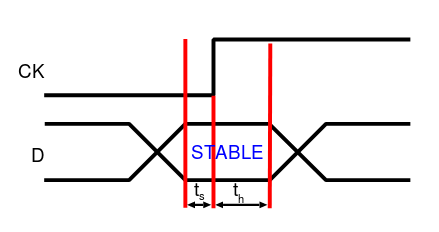
\includegraphics[width=8cm]{./ts_th.png}
  \begin{itemize}
    \itemsep0em
    \item $t_s$ le temps de résolution pour que la donnée passe à un état
    stable.
    \item $t_h$ le temps de front montant d'horloge où la donnée est stable.
    \item si $t_h \leq 0$, risque de métastabilité!
    \item MTBF : Mean Time Between Failure
  \end{itemize}
  \section{Mémoires}
  \begin{itemize}
    \itemsep0em
    \item ROM : Read-Only Memory
    \item RAM : Random Access Memory
    \item ROM = RAM, exemple de NON-RAM : bobine magnétique, carte perforée,etc
  \end{itemize}
  \subsection{Classification}
  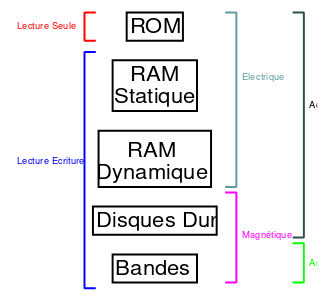
\includegraphics[width=8cm]{./mem_chart1.png}

  \newpage
  \begin{itemize}
    \itemsep0em
    \item bit : Binary digIT, plus petite quantité binaire
    \item octet : information codée sur 8 bits, unité binaire reférence
    \item mot : taille du bus de données
  \end{itemize}
  \begin{itemize}
    \itemsep0em
    \item Data Bus (M) : rend un mot de M bits depuis la mem.
    \item Addr Bus (N) : selectionne un mot parmi $2^N$.
    \item CS (Chip Select) : Activation du circuit
    \item R : Accès = lecture.
    \item W : Accès = écriture.
  \end{itemize}
  \subsection{Mémoires RAM}
  \subsubsection{Technologie SRAM}
  \begin{itemize}
    \itemsep0em
    \item Variante CAM : adressée par contenu (caches associatifs).
    \item Variante biport : Deux accès simultanés en mémoire.
  \end{itemize}
  Read:\\
  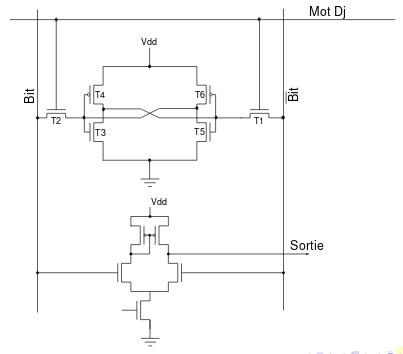
\includegraphics[height=6cm]{./sram_read.png}\\
  Write:\\
  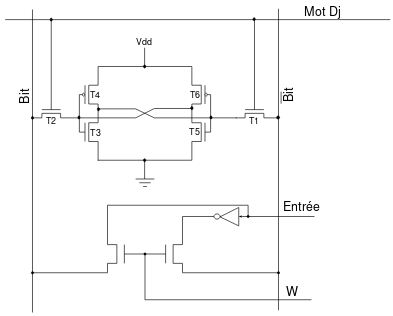
\includegraphics[height=6cm]{./sram_write.png}
  \begin{itemize}
    \itemsep0em
    \item \texttt{[+]} Rapide
    \item \texttt{[+/-]} Statique : rétention infinie tant qu'alimentée.
    \item \texttt{[+]} Techno CMOS : faible consommation.
    \item \texttt{[-]} Volumineuse.
    \item \texttt{[-]} Chère à produire.
    \item \texttt{[--]} Volatile.
  \end{itemize}
  \subsubsection{Technologie DRAM}
  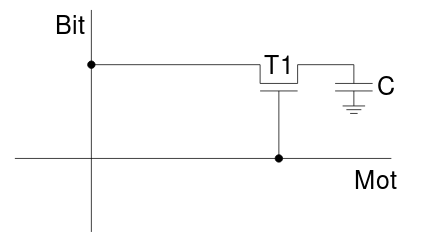
\includegraphics[width=8cm]{./dram_cell.png}
  \begin{itemize}
    \itemsep0em
    \item \texttt{[++]} Compact.
    \item \texttt{[+]} Techno CMOS : faible consommation.
    \item \texttt{[-]} Lecture destructrice : réecriture après lecture.
    \item \texttt{[-]} Déchargement du condensateur : rechargement régulier.
    \item \texttt{[--]} Volatile.
  \end{itemize}
  \subsubsection{Organisation interne}
  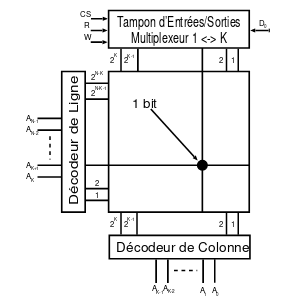
\includegraphics[width=8cm]{./internal_org.png}
  \subsubsection{Organisation externe}
  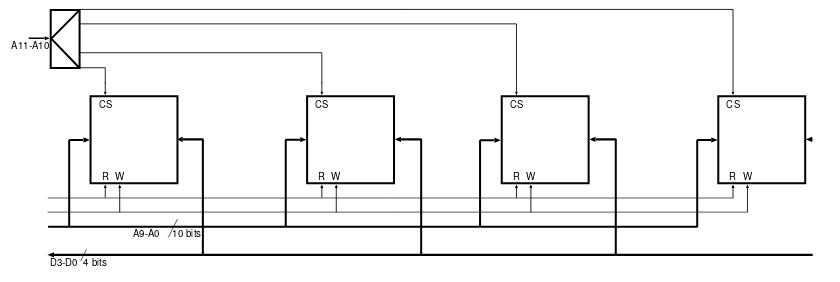
\includegraphics[width=10cm]{./external_org.png}
  \newpage
  \subsubsection{Technologie SDRAM}
  \begin{itemize}
    \itemsep0em
    \item Synchronous DRAM.
    \item Mémore candencée pour ne plus dépendre des délais matériels.
    \item Introduction du mode "rafale" (BURST)
  \end{itemize}
  \subsubsection{Technologie DDRAM}
  \begin{itemize}
    \itemsep0em
    \item Double-Rate DRAM.
    \item Lectures sur le front montant et descendant de l'horloge.
  \end{itemize}
  \subsubsection{Technologie QDRAM}
  \begin{itemize}
    \itemsep0em
    \item Quad-rate DRAM.
    \item Discossier Entrée de Sortie.\\
    $\rightarrow$ Lecture et écriture simultanée sur le cycle.
  \end{itemize}
  \subsection{Mémoires ROM}
  \begin{itemize}
    \itemsep0em
    \item Nécessité de mémoires non-volatile
    \item Ex: BIOS de $\mu$-ordinateurs.
    \item Ex2: stockage de programmes en systèmes embarqués.
  \end{itemize}
  \subsubsection{Types de ROM}
  \begin{itemize}
    \item Mask-ROM : réalisé lors de la fabrication du circuit.
    \item PROM : Programmable Read-Only Memory, programmable qu'une fois.
    \item EPROM : Erasable PROM, effacable par exposition à des rayons U.V.
    \item EEPROM : Ellectricaly EPROM, effacable électriquement.
    \item NOVRAM : RAM à alimentation indépendante (pile).
  \end{itemize}
  \section{Structure d'un FPGA}
  \begin{itemize}
    \itemsep0em
    \item FPGA sous-divisé en cellules.
    \begin{itemize}

    \itemsep0em
      \item LUT : Look-Up Tables (combinatoire).
      \item Bascules (séquentiel).
    \end{itemize}
    \item Entrées/Sorties.
    \item Logique de routage.
  \end{itemize}
  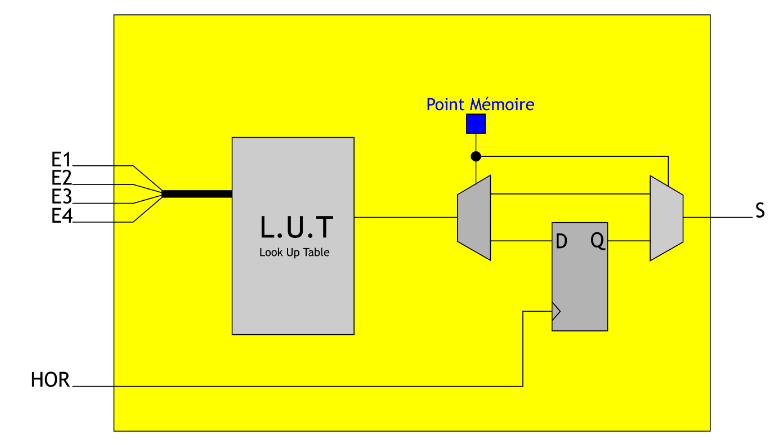
\includegraphics[width=8cm]{./lut.png}
  \section{Circuits reprogrammables/Tests}
  \subsection{Bed-Of-Nails}
  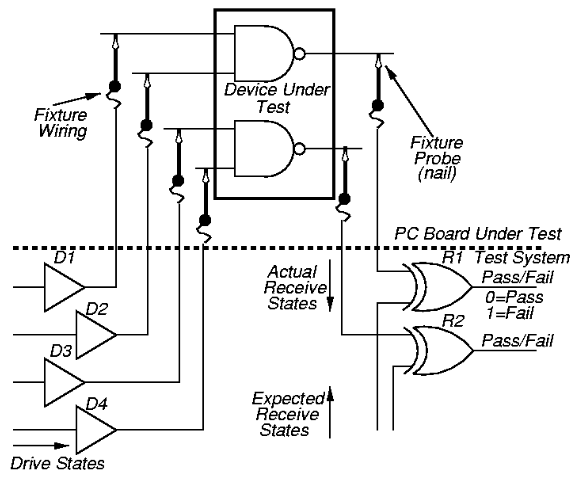
\includegraphics[width=8cm]{bon.png}
  \subsection{Boundary-Scan (JTAG)}
  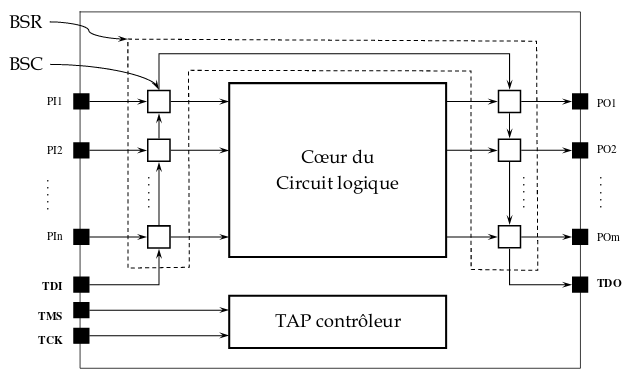
\includegraphics[width=8cm]{jtag1.png}
  JTAG : Joint Test Action Group\\
  Norme IEEE1149.1 : \textit{"Standard Test Access Port and Boundary-Scan
  Architecture"}
  \begin{itemize}
    \itemsep0em
    \item \texttt{[++]} Permet de tester des SoC.
    \item \texttt{[++]} Permet le In-System Programming des FPGA.
    \item \texttt{[++]} Permet de faire du diagnostic de circuit sans instrument
    supplémentaire.
    \item \texttt{[-]} Quatre plots obligatoires à ajouter à la carte.
    \item \texttt{[-]} Routage
    \item \texttt{[-]} Dégradation des délais.
    \item \texttt{[-]} Ralongement du TTM (Time-To-Market)
  \end{itemize}
  \newpage
  \subsubsection{Composition du Boundary Scan}
  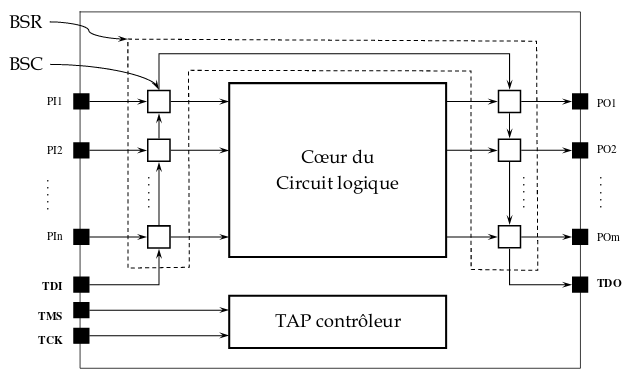
\includegraphics[width=8cm]{jtag1.png}
  \begin{itemize}
    \itemsep0em
    \item TCK : Horloge lors du Test.
    \item TMS : Test-Mode Select
    \item TDI : Test Data Input
    \item TDO : Test Data Output
  \end{itemize}
  \subsubsection{TAP Controller}
  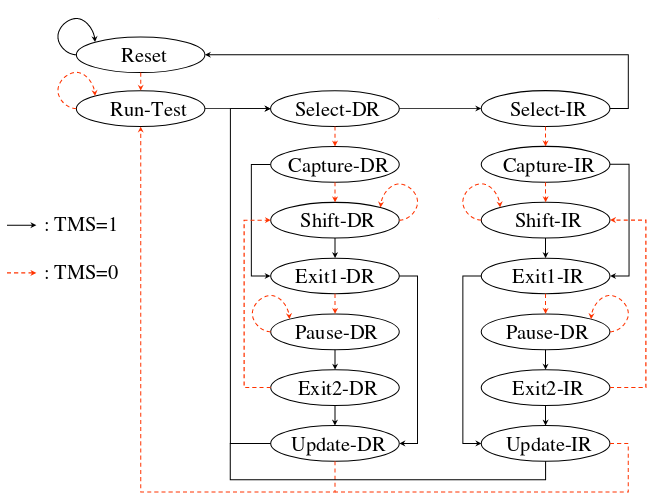
\includegraphics[width=8cm]{tap.png}
  \begin{itemize}
    \itemsep0em
    \item Test-Logic-Reset : État de Reset.
    \item Run-Test-Idle : Mise en attente.
    \item Select-IR/DR : Choix [Instr/Data/Reset].
    \item Capture-IR/DR : Le registre à décalage IR/DR est chargé en parallèle
    sur le front montant de TCK. Les valeurs sont décalées de l'entrée TDI vers
    la sortie TDO dans le registre à décalage IR/DR sur le front montant de TCK.
    \item Exit1-IR/DR : État temporaire.
    \item Pause-IR/DR : Attente de valeurs sur TDI.
    \item Exit2-IR/DR : État temporaire.
    \item Update-IR/DR : Les valeurs contenues du registre à décalage IR/DR sont
    chargées dans le registre parallèle IR/DR sur le front descendant de TCK.\\
    Prise en compte des nouvelles données par le circuit.
  \end{itemize}
  Remarques :
  \begin{itemize}
    \itemsep0em
    \item Si Etat=Shift-IR/DR $\rightarrow$ driver TDO activé.\\
          sinon $\rightarrow$ Haute Impédance.
    \item Les données sur TDI sont décalées sur le front montant de TCK, les
    données sont décalées à la fin de Shift-IR/DR.
    \item Les données sur TD0 sont décalées sur le front descendant de TCK, la
    donnée est présente sur TD0 $\dfrac{1}{2}$ cycle avant que la donnée sur TDI
    soit lue.
  \end{itemize}
  \subsubsection{Operations de IR}
  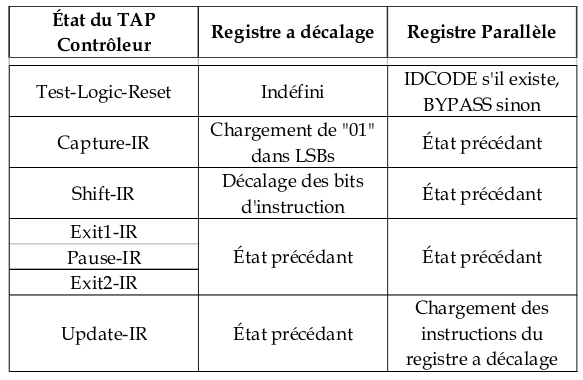
\includegraphics[width=8cm]{jtag_3.png}\\
  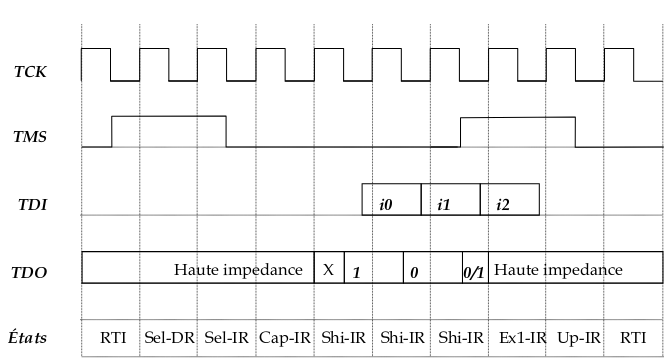
\includegraphics[width=8cm]{jtag_4.png}
  \subsubsection{Operations de DR}
  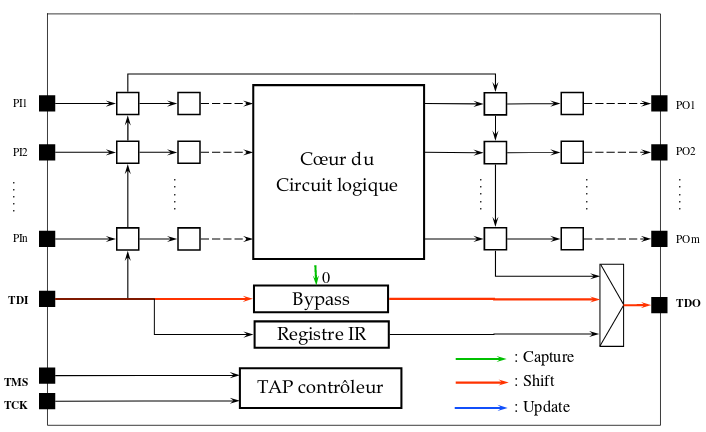
\includegraphics[width=8cm]{jtag_5.png}\\
  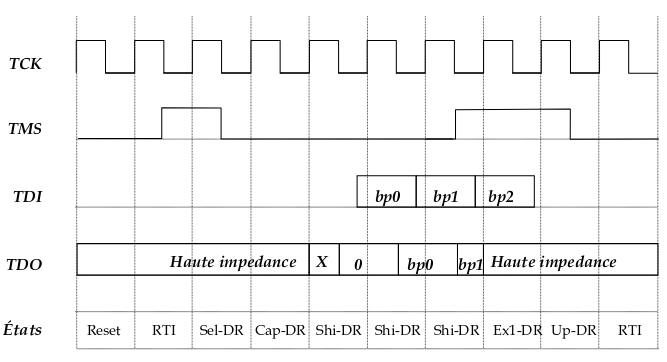
\includegraphics[width=8cm]{jtag_6.png}
  \newpage
  \subsubsection{EXTEST Mode}
  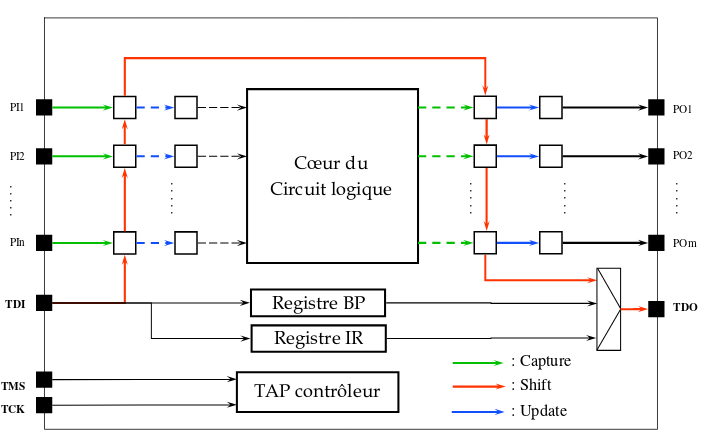
\includegraphics[width=8cm]{extest.png}\\
  Definitions :
  \begin{itemize}
    \itemsep0em
    \item PTV : Parallel Test Vector
    \item STV : Sequential Test Vector
    \item PRV : Parallel Response Vector
    \item SRV : Sequential Response Vector
  \end{itemize}
  Test en Boundary-Scan :
  \begin{enumerate}
    \itemsep0em
    \item Initialiser le TAP en mode Test-Logic-Reset.
    \item Charger l'instruction SAMPLE/PRELOAD.
    \item "Shift" le 1er vecteur STV.
    \item Charger l'instruction EXTEST.
    \item "Capture" la réponse du STV précedent dans le BSR.
    \item "Shift" la réponse SRV, en chargeant le vecteur suivant STV.
    \item "Update" le nouveau vecteur STV.
    \item Réitérer les étapes 5,6 \& 7 jusqu'au dernier vecteur STV.
    \item "Capture" la réponse du dernier vecteur STV.
    \item "Shift" la réponse SRV du dernier vecteur.
    \item Retourner à l'état Test-Logic-Reset.
  \end{enumerate}
  $\Rightarrow$ Tester les interconnexions entre les circuits d'une carte.
  \subsubsection{SAMPLE/PRELOAD Mode}
  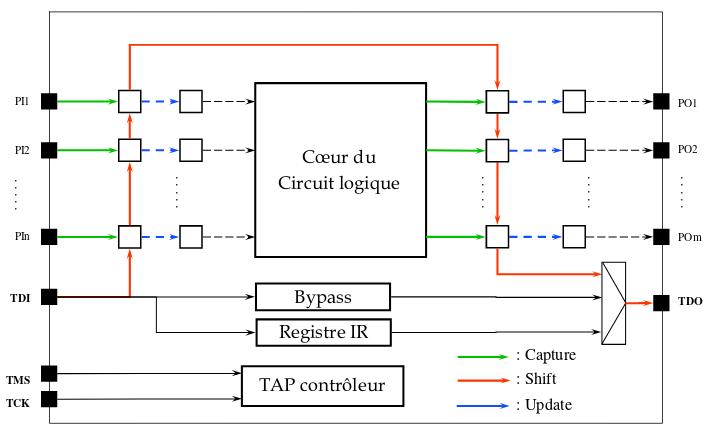
\includegraphics[width=8cm]{sample.png}\\
  $\Rightarrow$ Permet de pré-charger/echantilloner un circuit.
  \subsubsection{INTEST Mode}
  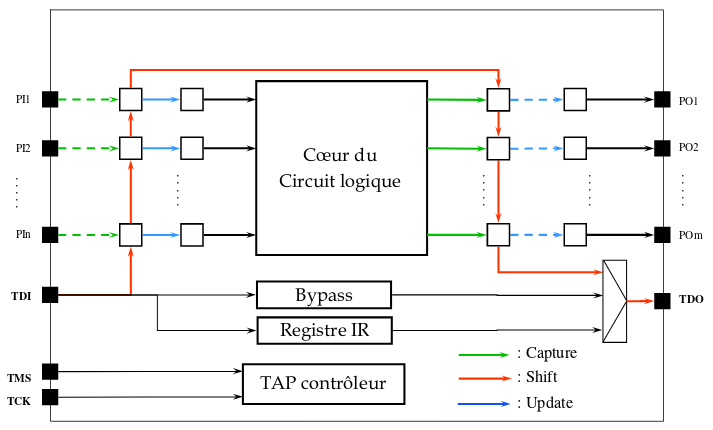
\includegraphics[width=8cm]{intest.png}\\
  Test en Boundary-Scan:
  \begin{itemize}
    \itemsep0em
    \item Selectionner le mode INTEST au lieu de EXTEST.
    \item Contrairement au mode EXTEST, les vecteurs sont à appliquer aux plots
    d'entrée du circuit et non aux plots de sortie.
    \item Les lecures sont à faire sur les plots de sortie du circuit et non aux
    plots d'entrées.
  \end{itemize}
  $\Rightarrow$ Isoler et tester indépendamment chaque circuit logique d'une
  carte.
  \subsubsection{RUNBIST Mode}
  \begin{enumerate}
    \itemsep0em
    \item Initialiser le TAP à Test-Logic-Reset.
    \item Charger l'instruction SAMPLE/PRELOAD.
    \item "Shift" le vecteur de sécurité
    \item Charger l'instruction RUNBIST, ce qui va selectionner le registre de
    sauvegarde de signature.
    \item Aller à l'étape Run-Test-Idle.
    \item Effectuer le nombre de coups d'horloge cécessaires pour le BIST.
    \item "Capture" le registre de signature.
    \item "Shift" la signature pour vérification.
    \item Revenir à l'état Test-Logic-Reset.
  \end{enumerate}
  $\Rightarrow$ RUNBIST : RUN Built-In Self-Test
  \vfill
  % If you were desperate about your exam to come across this, good luck! :)
  \hrule\vspace{.5em}
  \noindent Kevin Mambu\\
  M1 SESI 2017/2018\\
  \url{kev.mambu@protonmail.com}\\[1em]
  \hrule\vspace{.5em}
  \noindent\underline{\textbf{Sources}} :\\
  \textit{
  \textbf{Bertrand Granado} - Support de cours de Sysprog 2014\\
  \textbf{Alain Vachoux} - Le langage VHDL\\
  \textbf{Abdelhakim Khouas} - Conception en vue du Test : Le Boundary Scan}
\end{multicols}
\newpage
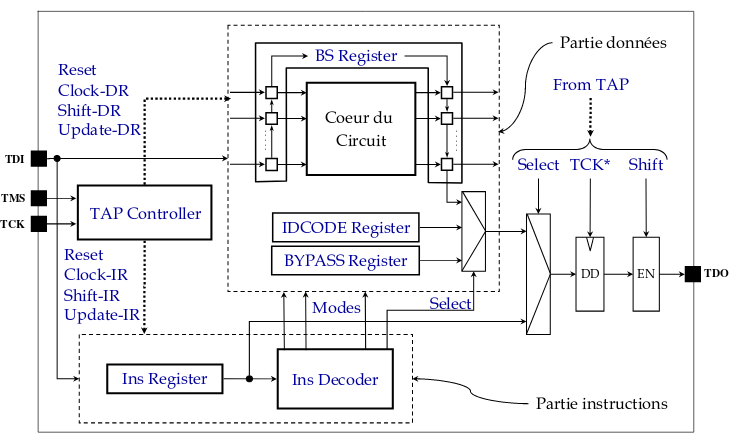
\includegraphics[angle=90]{fatman.png}
\end{document}
